\documentclass{beamer}
\setbeamertemplate{navigation symbols}{}


\usetheme{Montpellier}
\usepackage{lipsum}
\usepackage{graphicx}
\usepackage{amsmath}
\usepackage{mathtools}
\usepackage{amssymb}
\usepackage{bm}
\usepackage[utf8]{inputenc}


\begin{document}
	\title{Example-based Plastic Deformation of Rigid Bodies}   
	\author{Younes Müller} 
	\date{\today} 
	
	\frame{\titlepage} 
	
	\frame{\frametitle{Inhaltsverzeichnis}\tableofcontents} 
	
	\section{Einleitung}
	\frame{
		\frametitle{Flatout 2}
		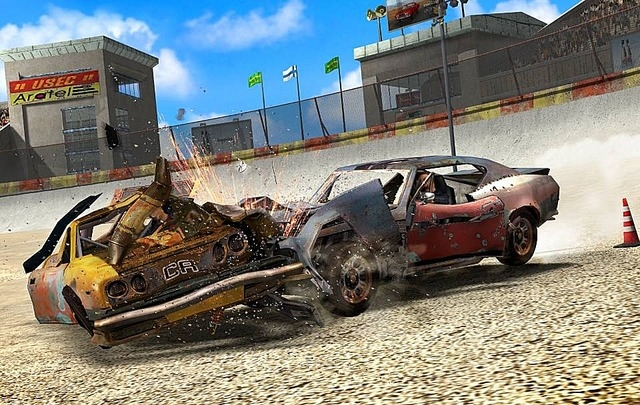
\includegraphics[width=.9\textwidth]{images/flatout2.jpg}\\
		\hyperlink{}{http://news.softpedia.com/images/reviews/large/flatout2ps2\_003-large.jpg}
	}
	\begin{frame}
		\begin{block}{Ziel}
			Effiziente Schadenssimulation
		\end{block}
		\begin{itemize}
			\item a
		\end{itemize}
	\end{frame}
	\section{Methode}
	\begin{frame}
		\frametitle{Methode}
	\end{frame}
	\subsection{Rigid Body Simulation}
	\begin{frame}
		\frametitle{Rigid Body Simulation}
	\end{frame}
	\subsection{Projection}
	\begin{frame}
		\frametitle{Projection}
	\end{frame}
	\subsection{Propagation}
	\begin{frame}
		\frametitle{Propagation}
	\end{frame}
	\subsection{Application}
	\begin{frame}
		\frametitle{Application}
	\end{frame}
	

	\subsection{Bl\"ocke}
	\frame{\frametitle{Bl\"ocke}
		
		\begin{block}{Blocktitel}
			Blocktext 
		\end{block}
		
		\begin{exampleblock}{Blocktitel}
			Blocktext 
		\end{exampleblock}
		
		
		\begin{alertblock}{Blocktitel}
			Blocktext 
		\end{alertblock}
	}
\end{document}

